\subsection{Development Board}

The development board for this project is the Raspberry Pi 4 Model B \ref{fig:rasp}, considering it is one of the constraints identified in the analysis phase (\ref{subsection:requirements_constraints}). This board includes a 64-bit quad-core ARM processor, the BCM2711, multimedia and connection features, ressembling to a computer-like board that serves multiple applications. The following list show the Raspberry Pi 4 Model B main features:

\begin{itemize}
        \item 2GB LPDDR4-3200 SDRAM;
        \item 2.4 GHz and 5.0 GHz IEEE 802.11ac wireless, Bluetooth 5.0, BLE;
        \item Raspberry Pi standard 40 pin GPIO header;   
        \item 2 USB 3.0 ports and 2 USB 2.0 ports;
        \item 2 micro-HDMI ports;
        \item 1 display port (2-lane MIPI DSI);
        \item 1 camera port (2-lane MIPI CSI);
        \item 1 jack 3,5 mm port (4-pole stereo audio and composite video port);
		\item graphic support (OpenGL ES 3.1, Vulkan 1.0);
		\item Micro-SD card slot.
\end{itemize}

%\item Raspberry Pi standard 40 pin GPIO header (fully backwards compatible with previous boards)

% A raspberry é apenas uma board de desenvolvimento, não é o hw que usariamos numa aplicação final.

\begin{figure}[ht]
	\centering
	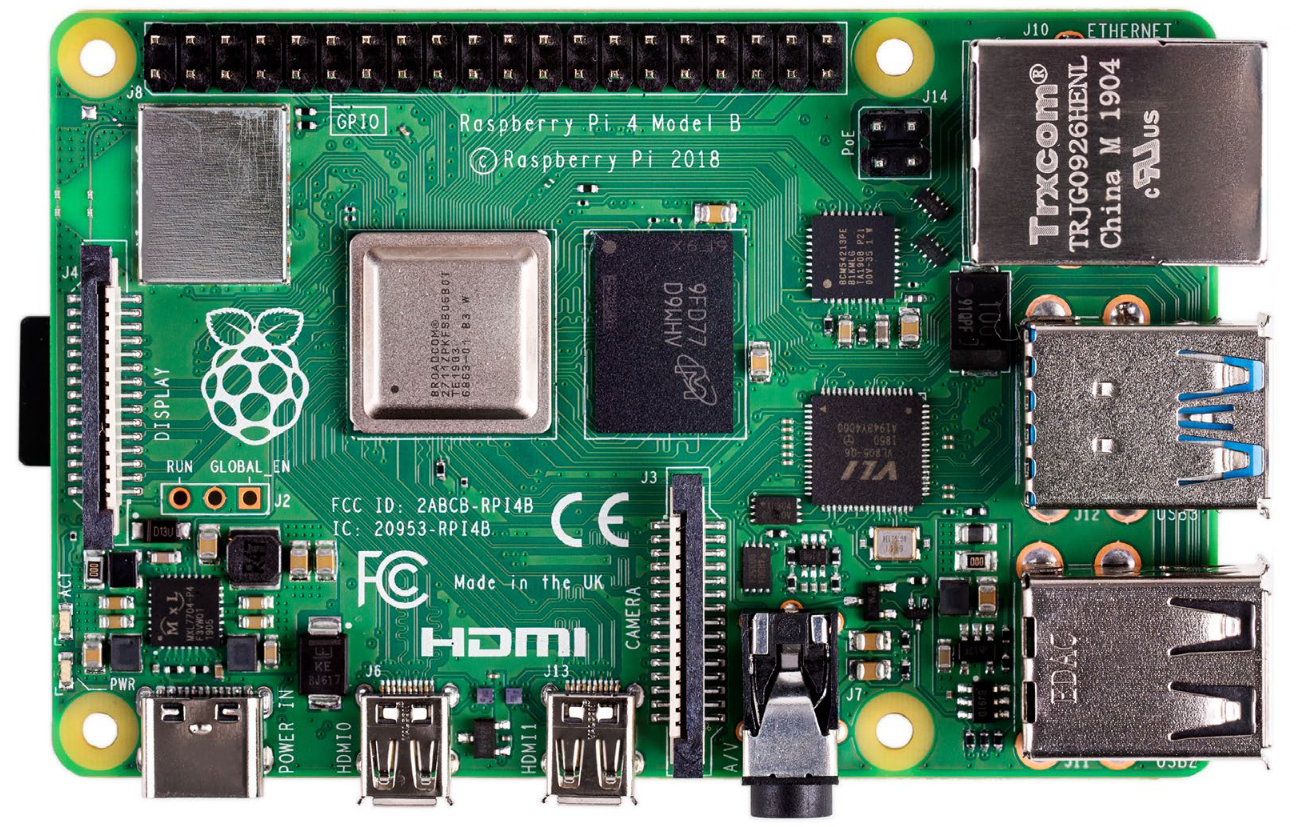
\includegraphics[width=.75\textwidth]{07hw_specification/raspberryPi}
	\caption{Raspberry Pi 4 Model B.}
	\label{fig:rasp}
\end{figure}

\subsubsection{\ac{gpio}}

The Raspberry Pi 4 Model B board comes with a standard 40 pin GPIO header, that allows to interface with external peripherals. This GPIO also provides some interface technologys, like UART, I2C or SPI. The GPIO pinout of this board is shown in figure \ref{fig:rasp_pinout} \cite{pinout}.

\begin{figure}[ht]
	\centering
	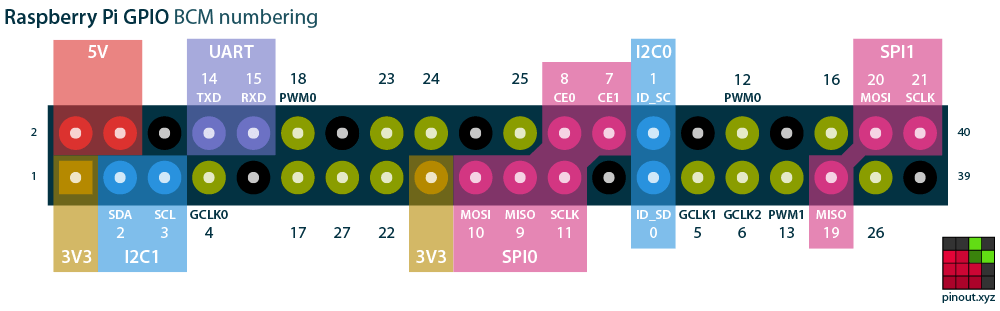
\includegraphics[width=1\textwidth]{07hw_specification/raspberryPi_pinout}
	\caption{Raspberry Pi 4 Model B GPIO Pinout.}
	\label{fig:rasp_pinout}
\end{figure}


\subsection{LED Lamp}

In order to light the streets efficiently, we must use a LED lamp. 

\subsection{Light Sensor}

In order to know when is night time, that is when the light conditions are low, one needs to determine the ambient light conditions, using a module composedby a \ac{ldr} sensor and a LM393 comparator, represented in figure \ref{fig:ldr}. The \ac{ldr} determines the environmental light conditions varying its resistivity. In the table \ref{table:ldr} is shown the LDR Module interface pins. When ambient light intensity does not reach the threshold value (defined by a potentiometer), the module's digital output (DO) is high, and when the ambient light level exceeds the threshold, the module's digital output terminal outputs low.

\begin{figure}[ht]
	\centering
	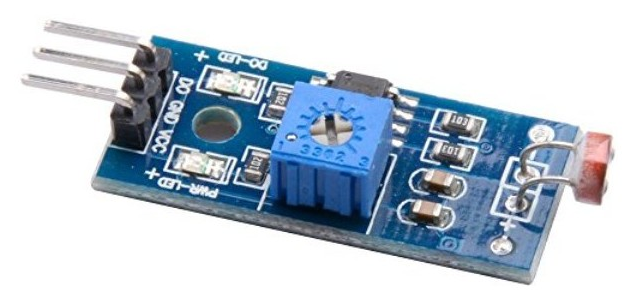
\includegraphics[width=0.70\textwidth]{07hw_specification/ldr}
	\caption{LDR Module.}
	\label{fig:ldr}
\end{figure}

\begin{table}[H]
	\centering
	\resizebox{0.5\columnwidth}{!}{
	\begin{tabular}{||c | c ||} 
		\hline
		\textbf{LDR Module Pin} & \textbf{Board Pin}\\\hline\hline
		VCC & 5 V\\\hline
		DO & Pin 17\\\hline
		GND & GND\\
		\hline
	\end{tabular}
	}		
	
	\caption{LDR Module Interface Pins.}
	\label{table:ldr}
\end{table}

\subsection{Movement Sensor}

To know when to turn on the light, it is necessary to detect movement in the streets. For this project it is used a movement sensor, more specifically a \ac{pir} sensor. The chosen sensor for this purpose was the PIR HC-SR501 that have a supply voltage range of 4,5 - 20 V and a detection range of 7 meters with a 110 degrees angle. In the table \ref{table:pir} is shown the PIR HC-SR501 interface pins, being the output signal the pin SIGNAL. When no movement is detected, the sensor output is low, and when movement is detected, the sensor SIGNAL is high. The sensor has also two potenciometers to adjust the trigger sensitivity and the delay of the trigger signal, between 0,3 seconds and 5 minutes.

\begin{figure}[H]
	\centering
	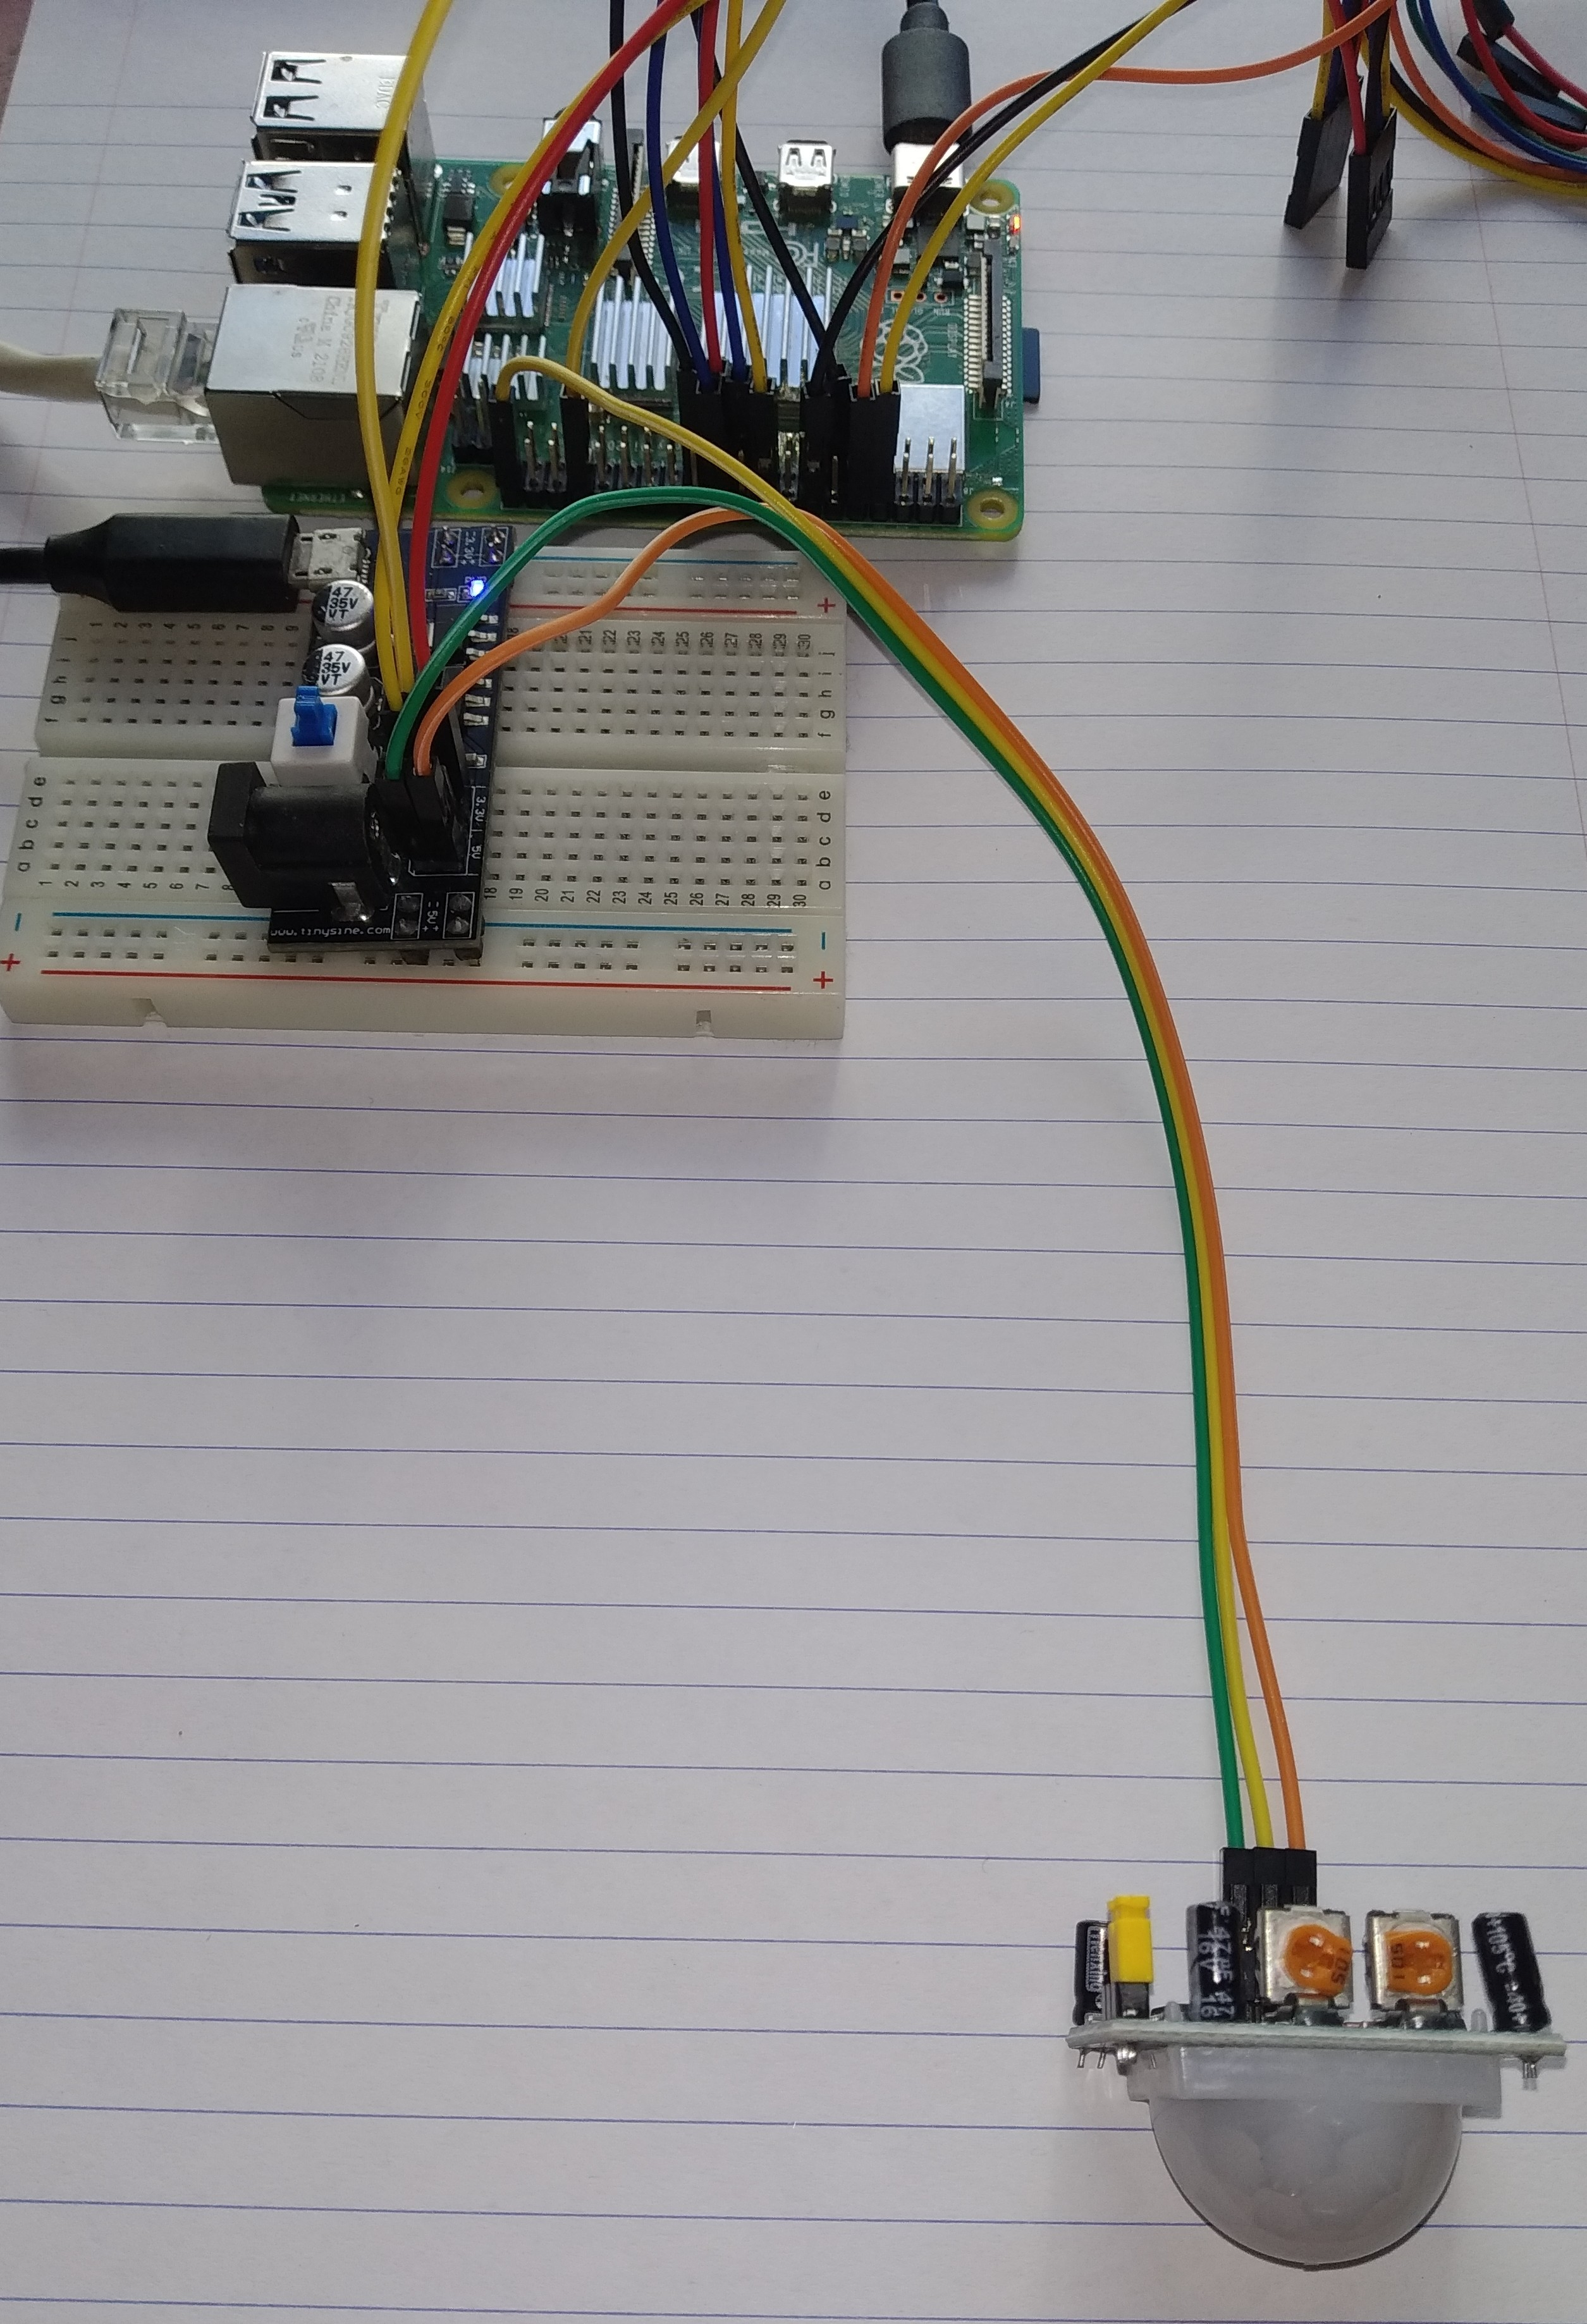
\includegraphics[width=0.70\textwidth]{07hw_specification/pir}
	\caption{PIR Sensor Module.}
	\label{fig:pir}
\end{figure}

\begin{table}[H]
	\centering
	\resizebox{0.5\columnwidth}{!}{
	\begin{tabular}{||c | c ||} 
		\hline
		\textbf{LDR Module Pin} & \textbf{Board Pin}\\\hline\hline
		VCC & 5 V\\\hline
		SIGNAL & Pin 27\\\hline
		GND & GND\\
		\hline
	\end{tabular}
	}		
	
	\caption{PIR Module Interface Pins.}
	\label{table:pir}
\end{table}